\section{Data application}
\label{sec:data}
\subsection{Adult income dataset}

The Census Income dataset, sometimes referred to as the Adult dataset, was extracted by \textcite{misc_adult_2} from the USA 1994 Census database. It has been widely used as a benchmark dataset in many machine learning research papers such as \textcite{poulos2018}, \textcite{chawla2002smote}, \textcite{menardi2014}, \textcite{yao2021review}, among others. It contains $48,842$ observations in total and includes $14$ regressors such as age, type of work (workclass), survey final weight (fnlwgt), level of education (education), number of years of education (education-num), marital status, occupation, relationship, race, sex, capital gain, capital loss, hours per week, native country, and income (class). The last one is the target value, where the purpose of the classification task is to predict whether the person will make more than $50$K per year.\\

This dataset is an ideal choice for a real-world dataset application within the frame of this thesis for two main reasons. Firstly, it contains a large number of observations, making it a popular subject in the research area of optimal subsampling methods for handling massive data, as demonstrated by studies such as \textcite{wang2018optimal} and \textcite{yao2021review}. Secondly, the data contains a moderate to high marginal imbalance, with $P(Y=1) \approx 0.25$. For the regression analysis, I follow \textcite{yao2021review} and use $5$ out of the $14$ features as relevant regressors for predicting $y$. After removing missing data, the sample consists of $N=45,222$ instances, where $11,208$ of them belong to class $Y=1$, i.e., adults who earned more than $50$K per year in 1994. Table \ref{tab:data-summary} provides summary statistics of the full sample used for the analysis, and additional summary statistics by class can be found in Section \ref{app:additional-tables}.

\begin{table}[ht] \centering 
\begin{tabular}{@{\extracolsep{5pt}}lccccc} 
\\[-1.8ex]\hline 
\hline \\[-1.8ex] 
Statistic & \multicolumn{1}{c}{N} & \multicolumn{1}{c}{Mean} & \multicolumn{1}{c}{St. Dev.} & \multicolumn{1}{c}{Min} & \multicolumn{1}{c}{Max} \\ 
\hline \\[-1.8ex] 
age & 45,222 & 38.548 & 13.218 & 17 & 90 \\ 
fnlwgt & 45,222 & 189,734.700 & 105,639.200 & 13,492 & 1,490,400 \\ 
education\_num & 45,222 & 10.118 & 2.553 & 1 & 16 \\ 
capital\_gain & 45,222 & 1,101.430 & 7,506.430 & 0 & 99,999 \\ 
capital\_loss & 45,222 & 88.595 & 404.956 & 0 & 4,356 \\ 
hours\_per\_week & 45,222 & 40.938 & 12.008 & 1 & 99 \\ 
class\_1 & 11,208 & 1.000 & 0.000 & 1 & 1 \\ 
class\_0 & 34,014 & 1.000 & 0.000 & 1 & 1 \\ 
\hline \\[-1.8ex] 
\end{tabular} 
\caption{Summary Statistics - Income dataset (missing values removed)} 
\label{tab:data-summary}
\end{table} 

One of the challenges is to determine whether or not there is conditional imbalance in the data. To address this, I visually analyze the PCA components as in Section \ref{sec:sim_general}. This can help identify whether the data clusters of each class overlap or not, which in turn could be an indicator of the presence of conditional imbalance. For instance, when the clusters cannot be fully separated by a hyperplane but are still distinguishable between them, it is possible that there exists conditional imbalance, which means that the probabilities of $P(Y=1)$ for certain feature values can be easily predicted. Figure \ref{fig:pca-data} illustrates the PCA components for each class, which appear dense due to the high number of observations. However, from the visualization, it is clear that there is a significant amount of class overlap, suggesting that this may be a case of mild-to-high marginal imbalance but low conditional imbalance, similar to the second numerical exercise of Simulation \ref{sec:sim4}.


\begin{figure}[ht]
    \centering
    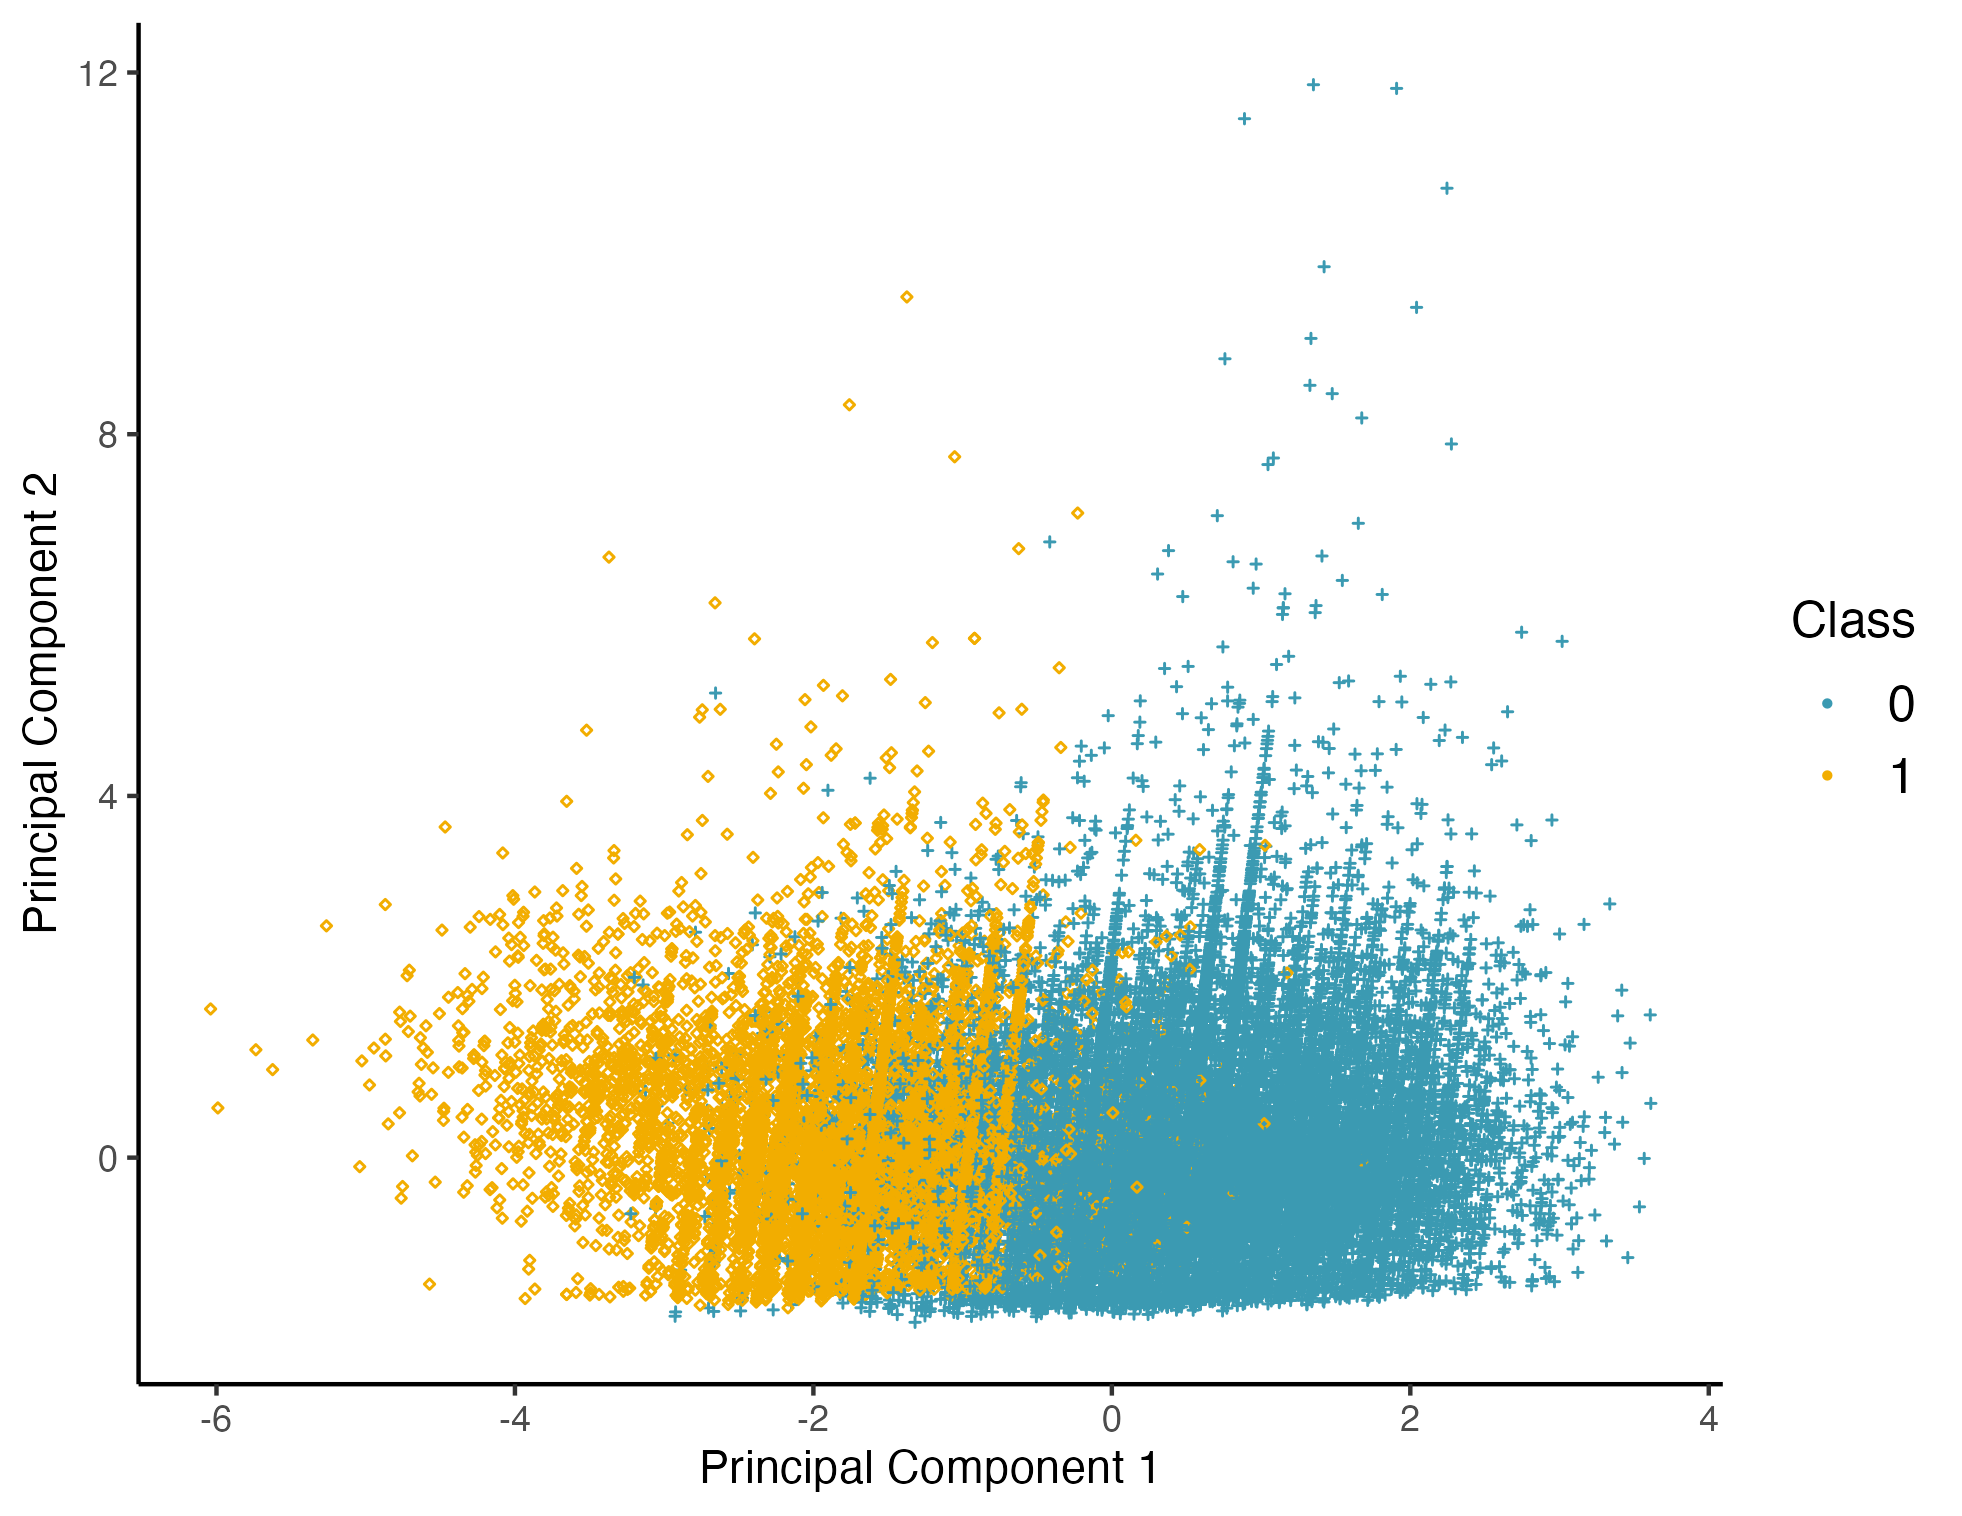
\includegraphics[scale=0.6]{2_Figures/plot_pca_data.png}
    \caption[Data application - PCA plot Income dataset]{PCA plot Income dataset (\cite{misc_adult_2}).}
    \label{fig:pca-data}
\end{figure}
